\section{Chase-Lev work-stealing deque}

\begin{frame}{Work-stealing}
\centering
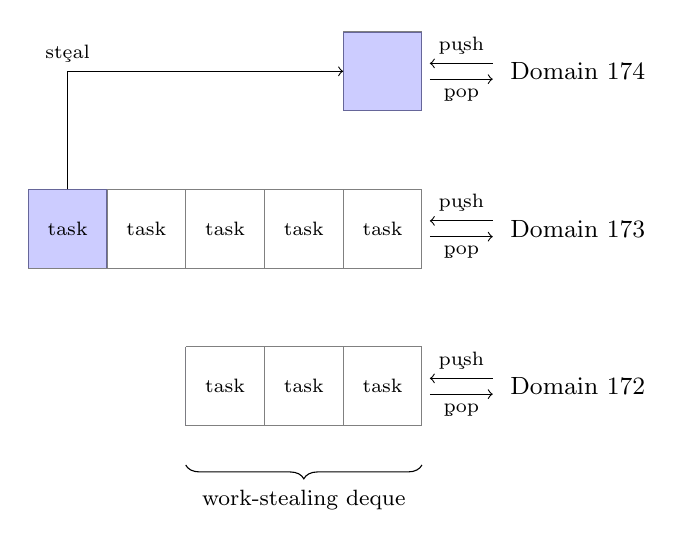
\begin{tikzpicture}
  \def\sep{1}
  \def\hsep{0.1}
  \def\vsep{0.4}
  \def\lenI{3}
  \def\lenxI{0}
  \def\lenII{4}
  \def\lenxII{1}
  \def\lenIII{0}
  \def\lenxIII{1}

  \node [right] at (1, 0.5) {\small Domain \ding{172}} ;
  \draw [step=1cm, gray] (0, 0) grid ++(-\lenI, 1) ;
  \draw [step=1cm, gray] (-\lenI, 0) grid ++(-\lenxI, 1) ;
  \fill [blue, opacity=0.2] (-\lenI, 0) rectangle ++(-\lenxI, 1) ;
  \draw [decorate, decoration={brace, amplitude=5pt}] (0, -0.5) -- ++(-\lenI, 0) node [midway, below, yshift=-2mm] {\footnotesize work-stealing deque} ;
  \draw [->] (\hsep, \vsep) -- ++(1 - 2 * \hsep, 0) node[midway, below] {\scriptsize\c{pop}} ;
  \draw [->] (1 - \hsep, 1 - \vsep) -- ++(2 * \hsep - 1, 0) node[midway, above] {\scriptsize\c{push}} ;
  \foreach \x in {1, ..., \lenI} {
  	\node at (0.5 - \x, 0.5) {\scriptsize task} ;
  }

  \node [right] at (1, \sep + 1.5) {\small Domain \ding{173}} ;
  \draw [step=1cm, gray] (0, \sep + 1) grid ++(-\lenII, 1) ;
  \draw [step=1cm, gray] (-\lenII, \sep + 1) grid ++(-\lenxII, 1) ;
  \fill [blue, opacity=0.2] (-\lenII, \sep + 1) rectangle ++(-\lenxII, 1) ;
  \draw [->] (\hsep, \sep + 1 + \vsep) -- ++(1 - 2 * \hsep, 0) node[midway, below] {\scriptsize\c{pop}} ;
  \draw [->] (1 - \hsep, \sep + 2 - \vsep) -- ++(2 * \hsep - 1, 0) node[midway, above] {\scriptsize\c{push}} ;
  \foreach \x in {1, ..., \lenII} {
  	\node at (0.5 - \x, \sep + 1.5) {\scriptsize task} ;
  }
  \node at (0.5 - \lenII - \lenxII, \sep + 1.5) {\scriptsize task} ;

  \node [right] at (1, 2 * \sep + 2.5) {\small Domain \ding{174}} ;
  \draw [step=1cm, gray] (0, 2 * \sep + 2) grid ++(-\lenIII, 1) ;
  \draw [step=1cm, gray] (-\lenIII, 2 * \sep + 2) grid ++(-\lenxIII, 1) ;
  \fill [blue, opacity=0.2] (-\lenIII, 2 * \sep + 2) rectangle ++(-\lenxIII, 1) ;
  \draw [->] (\hsep, 2 * \sep + 2 + \vsep) -- ++(1 - 2 * \hsep, 0) node[midway, below] {\scriptsize\c{pop}} ;
  \draw [->] (1 - \hsep, 2 * \sep + 3 - \vsep) -- ++(2 * \hsep - 1, 0) node[midway, above] {\scriptsize\c{push}} ;

  \draw [->, to path={|- node[above] {\scriptsize\c{steal}} (\tikztotarget)}] (0.5 - \lenII - \lenxII, \sep + 2) to (- \lenIII - \lenxIII, 2 * \sep + 2.5) ;
\end{tikzpicture}

\end{frame}

\begin{frame}{Chase-Lev work-stealing deque}
\centering
\includegraphics[scale=.5]{images/chaselev_paper.pdf}
\end{frame}

% simplified version with one infinite array (as opposed to multiple circular arrays)
\begin{frame}{Physical state}
\centering
\large
\scalebox{1.2}{
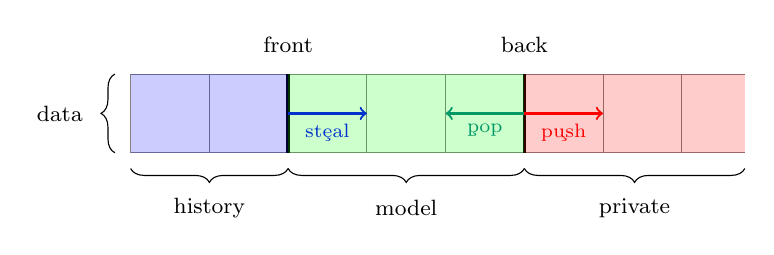
\begin{tikzpicture}
  \def\history{2}
  \def\model{3}
  \def\private{2.8}

  \visible<1->{
    \draw [step=1cm, gray] (0,0) grid ++(\history+\model+\private,1) ;
    \draw [decorate, decoration={brace, amplitude=5pt}] (-.2,0) -- ++(0,1) node [midway, xshift=-7mm] {\footnotesize data} ;
  }

  \visible<2->{
    \draw [very thick] (\history,0) -- ++(0,1) node [label=above:\footnotesize front] {} ;
    \draw [thick, ->, blue] (\history,.5) -- ++(1,0) node [midway, below] {\scriptsize\c{steal}} ;
  }
  
  \visible<3->{
    \draw [very thick] (\history+\model,0) -- ++(0,1) node [label=above:\footnotesize back] {} ;
    \draw [thick, ->, teal] (\history+\model,.5) -- ++(-1,0) node [midway, below] {\scriptsize\c{pop}} ;
    \draw [thick, ->, red] (\history+\model,.5) -- ++(1,0) node [midway, below] {\scriptsize\c{push}} ;
  }
  
  \visible<4->{
    \fill [blue, opacity=.2] (0,0) rectangle ++(\history,1) ;
    \draw [decorate, decoration={brace, amplitude=5pt}] (\history,-.2) -- ++(-\history,0) node [midway, yshift=-5mm] {\footnotesize history} ;
  }
  
  \visible<5->{
    \fill [green, opacity=.2] (\history,0) rectangle ++(\model,1) ;
    \draw [decorate, decoration={brace, amplitude=5pt}] (\history+\model,-.2) -- ++(-\model,0) node [midway, yshift=-5mm] {\footnotesize model} ;
  }
  
  \visible<6->{
    \fill [red, opacity=.2] (\history+\model,0) rectangle ++(\private,1) ;
    \draw [decorate, decoration={brace, amplitude=5pt}] (\history+\model +\private,-.2) -- ++(-\private,0) node [midway, yshift=-5mm] {\footnotesize private} ;
  }
\end{tikzpicture}
}

\vfill

\begin{tabular}{r@{:\hskip1em}l}
  \visible<1->{
      data &
      infinite array storing all values
  }
  \visible<2->{
    \\
      front &
      \emph{monotonic} thieves' index
  }
  \visible<3->{
    \\
      back &
      owner's index
  }
  \visible<4->{
    \\
      history &
      \emph{monotonic} list of values
  }
  \visible<5->{
    \\
      model &
      logical content of the deque
  }
  \visible<6->{
    \\
      private &
      owner-only region
  }
\end{tabular}

\end{frame}

% external future-dependent linearization point
\begin{frame}{Logical state}
\centering
\scalebox{.9}{
\begin{tikzpicture}
  \def\width{4cm}
  \def\height{2cm}

  \visible<1->{
    \node [align=center] (s1) {
      \ding{172} Empty \\
    	\begin{tikzpicture}[scale=.5]
        \def\hist{2}
        \def\priv{2.8}
  
        \draw [step=1cm, gray] (0,0) grid (\hist+\priv,1) ;
  
        \fill [blue, opacity=.2] (0,0) rectangle (\hist,1) ;
        \draw [very thick] (\hist,1) -- ++(0,-1) node [yshift=2mm, label=below:{\tiny front = back}] {} ;
        \fill [red, opacity=.2] (\hist,0) rectangle ++(\priv,1) ;
      \end{tikzpicture}
    } ;

    \node [align=center] (s2) [right=\width of s1] {
      \ding{173} Non-empty \\
      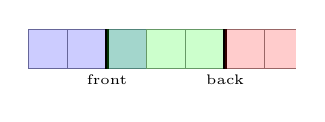
\begin{tikzpicture}[scale=.5]
        \def\hist{2}
        \def\histx{1}
        \def\model{3}
        \def\priv{1.8}
  
        \draw [step=1cm, gray] (0,0) grid (\hist+\model+\priv,1) ;
  
        \fill [blue, opacity=.2] (0,0) rectangle (\hist+\histx,1) ;
        \draw [very thick] (\hist,1) -- ++(0,-1) node [yshift=2mm, label=below:{\tiny front}] {} ;
        \fill [green, opacity=.2] (\hist,0) rectangle ++(\model,1) ;
        \draw [very thick] (\hist+\model,1) -- ++(0,-1) node [yshift=2mm, label=below:{\tiny back}] {} ;
        \fill [red, opacity=.2] (\hist+\model,0) rectangle ++(\priv,1) ;
      \end{tikzpicture}
    } ;
  }

  \visible<2->{
    \node [align=center] (s3) [below=\height of s2] {
      \ding{174} Emptyish \\
      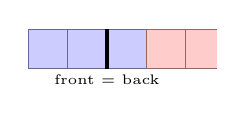
\begin{tikzpicture}[scale=.5]
        \def\hist{2}
        \def\histx{1}
        \def\priv{2.8}
  
        \draw [step=1cm, gray] (0,0) grid (\hist+\priv,1) ;
  
        \fill [blue, opacity=.2] (0,0) rectangle (\hist+\histx,1) ;
        \draw [very thick] (\hist,1) -- ++(0,-1) node [yshift=2mm, label=below:{\tiny front = back}] {} ;
        \fill [red, opacity=.2] (\hist+\histx,0) rectangle ++(\priv-\histx,1) ;
      \end{tikzpicture}
    } ;
    
    \node [align=center] (s4) [below=\height of s1] {
      \ding{175} Super-empty \\
      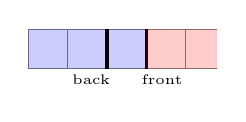
\begin{tikzpicture}[scale=.5]
        \def\hist{2}
        \def\histx{1}
        \def\priv{2.8}
  
        \draw [step=1cm, gray] (0,0) grid (\hist+\priv,1) ;
  
        \fill [blue, opacity=.2] (0,0) rectangle (\hist+\histx,1) ;
        \draw [very thick] (\hist,1) -- ++(0,-1) node [xshift=-2mm, yshift=2mm, label=below:{\tiny back}] {} ;
        \draw [very thick] (\hist+\histx,1) -- ++(0,-1) node [xshift=2mm, yshift=2mm, label=below:{\tiny front}] {} ;
        \fill [red, opacity=.2] (\hist+\histx,0) rectangle ++(\priv-\histx,1) ;
      \end{tikzpicture}
    } ;
  }

  \visible<3->{
    \draw [thick, ->] (s1) to [bend left] node [above] {\c{push}} (s2) ;
    \draw [thick, ->] (s2) to [bend left] node [below] {\c{steal}} (s1) ;
  \draw [thick, ->] (s2) to [looseness=3, out=135, in=45] node [above] {\c{push}, \c{pop}, \c{steal}} (s2) ;
  }
  
  \visible<4->{
    \draw [thick, ->] (s2) to [bend left] node [right] {\c{pop}} (s3) ;
  }
  
  \visible<5->{
    \draw [thick, dotted, ->] (s3) to [bend left] node [below] {\c{pop}, \c{steal}} (s4) ;
  }
  
  \visible<6->{
    \draw [thick, dotted, ->] (s4) to [bend left] node [left] {\c{pop}} (s1) ;
  }
  
  \visible<7->{
    \draw [thick, dotted, ->] (s1) to [bend left] node [right] {\c{pop}} (s4) ;
  }
  
  \visible<3->{
    \matrix [right, nodes={font=\tiny}] at (current bounding box.south west) {
      \draw [thick, ->] (0,0) -- (1em,0) node [right] {linearization} ; \\
      \draw [thick, dotted, ->] (0,0) -- (1em,0) node [right] {stabilization} ; \\
    } ;
  }
\end{tikzpicture}
}

\end{frame}

\begin{frame}{Prophecy variables / Prophets}
\large
\begin{itemize}
  \setlength\itemsep{1em}
  \item
    \textbf{Primitive prophets} \\
    Predict the future of the execution.
  \item
    \textbf{Typed prophets} \\
    Prediction belongs to a user-supplied semantic type.
  \item
    \textbf{\textcolor{color2}{Wise prophets}} \\
    Remember past predictions. \\
    Eliminate inconsistent branches.
  \item
    \textbf{\textcolor{color2}{Multiplexed prophets}} \\
    Separate logically independent predictions on a single prophet.
\end{itemize}
\end{frame}
